\documentclass{standalone}
\usepackage{tikz}
\begin{document}
 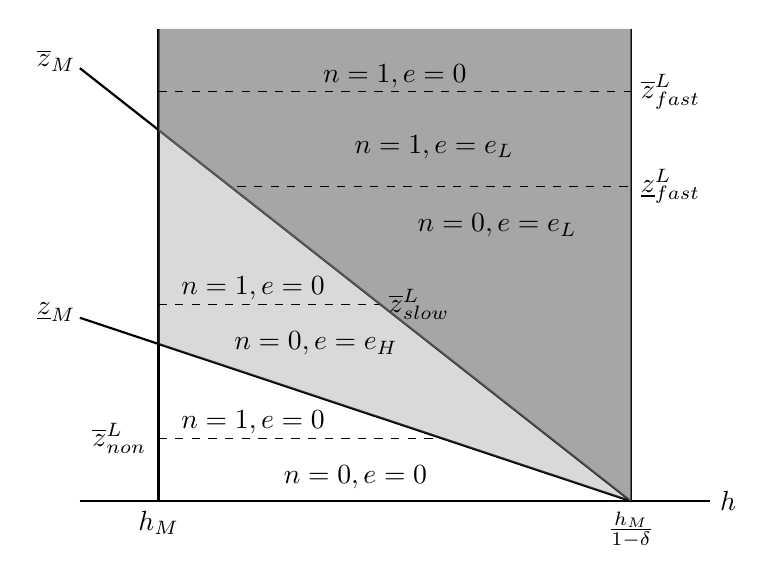
\begin{tikzpicture}

% Axes
\draw[thick] (-1,0) -- (7,0) node[right] {$h$};
% Vertical divisions
\draw[thick] (0,6) -- (0,0) node[below] {$h_M$};
\draw[thick] (6,6) -- (6,0) node[below] {$\frac{h_M}{1-\delta}$};




% Diagonal lines
\draw[thick] (-1,5.5) -- (6,0) ;
\draw[thick] (-1,2.33) -- (6,0);
\node at (-1.3,5.6) {$\overline{z}_M$};
\node at (-1.3,2.4) {$\underline{z}_M$};

% Shade the area between the diagonal lines and the left vertical line
\fill[gray, opacity=0.3] 
    (0,2) -- (0,4.7) -- (6,0) -- cycle;
\fill[gray, opacity=0.7] 
    (0,4.7) -- (0,6) -- (6,6) -- (6,0) -- cycle;

% Horizontal lines
\draw[dashed] (0,5.2) -- (6,5.2) node[right] {$\overline{z}^L_{fast}$};% First top dashed line bounded by diagonal
\draw[dashed] (1,4) -- (6,4) node[right] {$\underline{z}^L_{fast}$}; % Second top dashed line bounded by top diagonal and vertical line
\draw[dashed] (0,2.5) -- (2.8,2.5) node[right] {$\overline{z}^L_{slow}$}; % Third dashed line bounded by vertical line and top diagonal
\draw[dashed] (0,0.8) -- (3.6,0.8) ; % Bottom dashed line bounded by diagonal line

% Labels


\node at (-0.5,0.8) {$\overline{z}^L_{non}$};

% Region Labels
\node at (3,5.4) {$n=1, e=0$};
\node at (3.5,4.5) {$n=1, e=e_L$};
\node at (4.3,3.5) {$n=0, e=e_L$};

\node at (1.2,2.7) {$n=1, e=0$};
\node at (2,2) {$n=0, e=e_H$};

\node at (1.2,1) {$n=1, e=0$};
\node at (2.5,0.3) {$n=0, e=0$};

\end{tikzpicture}


\end{document}
